
\chapter{La ricerca}
	Un altro problema fondamentale dei siti è far sì che il proprio contenuto sia trovato dagli utenti. La ricerca diviene quindi un fattore fondamentale all'interno del web. Esistono varie modalità di ricerca, prima di tutto ogni sito internet se abbastanza grande dovrebbe avere come servizio la ricerca interna vedremo come inserirla nel nostro sito garantendo l'usabilità ed discutendo problemi di molti siti. Scopriremo anche i motivi per cui diverse modalità di ricerca al primo impatto stupefacenti si rivelano essere fallimentari per l'usabilità dei siti internet. Sono le ricerche 2.0 che con numerosi tentativi negli anni hanno cercato di sfruttare la sintesi vocale lottando contro il problema del contesto.

	\section{Ricerca interna}
		Una ricerca interna al proprio sito e la qualità di essa è determinata dal numero di pagine che questo ha.
		\begin{itemize}
			\item \textbf{>100} è \textbf{necessario} che il sito abbia uno strumento di ricerca.
			\item \textbf{>1000} è \textbf{cruciale} che lo strumento di ricerca sia buono.
		\end{itemize}
		Si stima che la ricerca è utilizzata quasi nel 100\% dei casi. Gli utenti sono abituati ai motori di ricerca e molto spesso gli utenti arrivano in una pagina qualunque del sito attraverso il \emph{deep linking}. Difatti:
		\begin{itemize}
			\item il 60\% usa la ricerca appena giunge in un sito (se essa è disponibile).
			\item il 40\% fa uso di link.
		\end{itemize}
		
		Vista l'enorme importanza in molti siti si tende ad inserire uno strumento di ricerca, ma questo se fatto come si deve è molto costoso e troppo spesso si incorre all'uso di soluzioni \emph{low cost} che peggiorano soltanto la situazione. Solitamnete questa soluzione è di localizzare motori di ricerca sul proprio sito: costo zero ma:
		\begin{itemize}
			\item l'algoritmo dei motori di ricerca è ottimizzato per larghe scale, su bassa scala non dà risultati soddisfacenti.
			\item Se l'utente usa la ricerca significa molto probabilmente che il motore di ricerca già utilizzato non l'ha portato al suo scopo per cui utilizzarlo ancora non servirà a niente.
			\item I motori di ricerca non fanno la lettura di tutte le pagine (il 70\% del web è sconosciuto ai motori di ricerca) per cui questo può far sì che alcune pagine del sito non compariranno mai tra i risultati.
		\end{itemize}			
	
		\subsection{Ricerca su misura}	
			Gli utenti preferiscono:
			\begin{itemize}
				\item 1 sola modalità di ricerca come i motori di ricerca.
				\item Un \textbf{box testuale} e un \textbf{pulsante} con scritto "search" (o "cerca"). Null'altro è da sostituire alla parola "search".
				\item Si può sostituire il box testuale e il pulsante con l'icona della lente per siti mobile. In generale però gli utenti preferiscono sempre il testo.
			\end{itemize}
	
			\subsubsection{Principio di Robert Browning}
				Enunciamo un principio che nel web ha praticamente valenza generale. IL primo ad nunciarlo fu Robert Browning e in seguito fu ripreso dall'architetto modernista Ludwig Mies van der Rohe.
				\begin{quote}
					``\emph{Less is more}''
				\end{quote}
				Che applicato al web consiste in: \emph{meno dettagli e orpelli significa qualcosa di meglio}. L'esempio lampante è la pagina iniziale del motore di ricerca Google.
				Ludwig Mies van der Rohe estese anche il principio in:
				\begin{quote}
					``\emph{Less is more but God is in the detail}''
				\end{quote} 
				Per capire quanto i dettagli sono importanti si veda l'Errore 404 spiegato successivamente.
	
	\section{Ricerca vincolata}
		La ricerca vincolata si prefigge di accompagnare l'utente passo passo attraverso parametri, deve essere considerata come un'aggiunta alla classica ricerca spiegata in precedenza. Vantaggi e svantaggi:
		\begin{itemize}
			\item è efficiente e gradita dagli utenti.
			\item esistono due modalità di come si offre ognuna con i suoi svantaggi.
		\end{itemize}
		
					
		\subsection{Ricerca vincolata dinamica}
			La ricerca dinamica avviene per ogni settaggio di un parametro.
			Svantaggi:
			\begin{itemize}
				\item Quando il numero dei vincoli è tanto l'attesa del caricamento è alto.
				\item Abbiamo un carico del server notevolmente maggiore.
				\item Se l'utente ha già i vincoli in mente dovrà fare comunque più ricerche.
			\end{itemize}
	
		\subsection{Ricerca vincolata statica}
			La ricerca avviene solo nel momento in cui l'utente ha impostato tuti i parametri richiesti e ha dato il via.
			Svantaggi:
			\begin{itemize}
				\item Il pulsante non ha contenuto standard. Le parole "search" o "cerca" illudono che sia la ricerca classica. 
				\item Se un utente è abituato a quella dinamica resta confuso al prima impostazione di parametro perché non succede nulla. Questo può indurlo a pensare che non funzioni.
			\end{itemize}
		
		\subsection{Soluzione ibrida}
			In generale la soluzione dinamica è meglio nel caso in cui un utente non sappia cosa cercare mentre p il contrario per la ricerca statica. Esiste una terza soluzione che consiste nell'avviare la ricerca automaticamente al termine del settaggio dei parametri. In questo modo togliamo il pulsante per la ricerca statica e non appesantiamo il server con ricerche in più.
		
	\section{Consigli}
		DI seguito elenchiamo alcuni consigli per mostrare i risultati di ricerca nel migliore dei modi.
		\begin{description}
			\item[Ordinamento:] mettere sempre a disposizione un ordinamento bidirezionale.
			\item[Casi limite:] se non ci sono risultati dobbiamo comunicare all'utente che ci non ci sono risultanti altrimenti si confonde l'utente che pensa non funzioni.
			\item[Error 404:] quando i link sono "rotti" (non esistono più) deve esserci una pagina con suggerimenti all'utente che offrono aiuto. Molte volte a queste si affianca qualcosa di simpatico che ironizza la situazione, ciò sospende i timer, un esempio di questo lo troviamo nella pagina 404 del sito \href{http://www.b3ta.com/error404}{www.b3ta.com}, che raccoglie le più esilaranti immagini delle pagine error 404 nel web.
			\item[Presentazione risultati:] esistono due modi per presentare i risultati di una ricerca.
				\begin{itemize}
					\item Modalità classica: vedi figura ~\ref{fig:LaRicerca-Consigli}.
					\item Modalità a griglia: permette di visualizzare molta più informazione compatta ma questo fa sì che gli elementi mostrati perdano rilevanza. Con questa modalità l'utente si confonde e si perde nella micro-navigazione. Non a caso Google immagini propone i risultati a griglia, vuole che l'utente stia per più tempo all'interno del sul otore di ricerca. (vedi figira ~\ref{fig:LaRicerca-Consigli})
				\end{itemize}
		\end{description}
		
		\begin{figure}
			\centering
			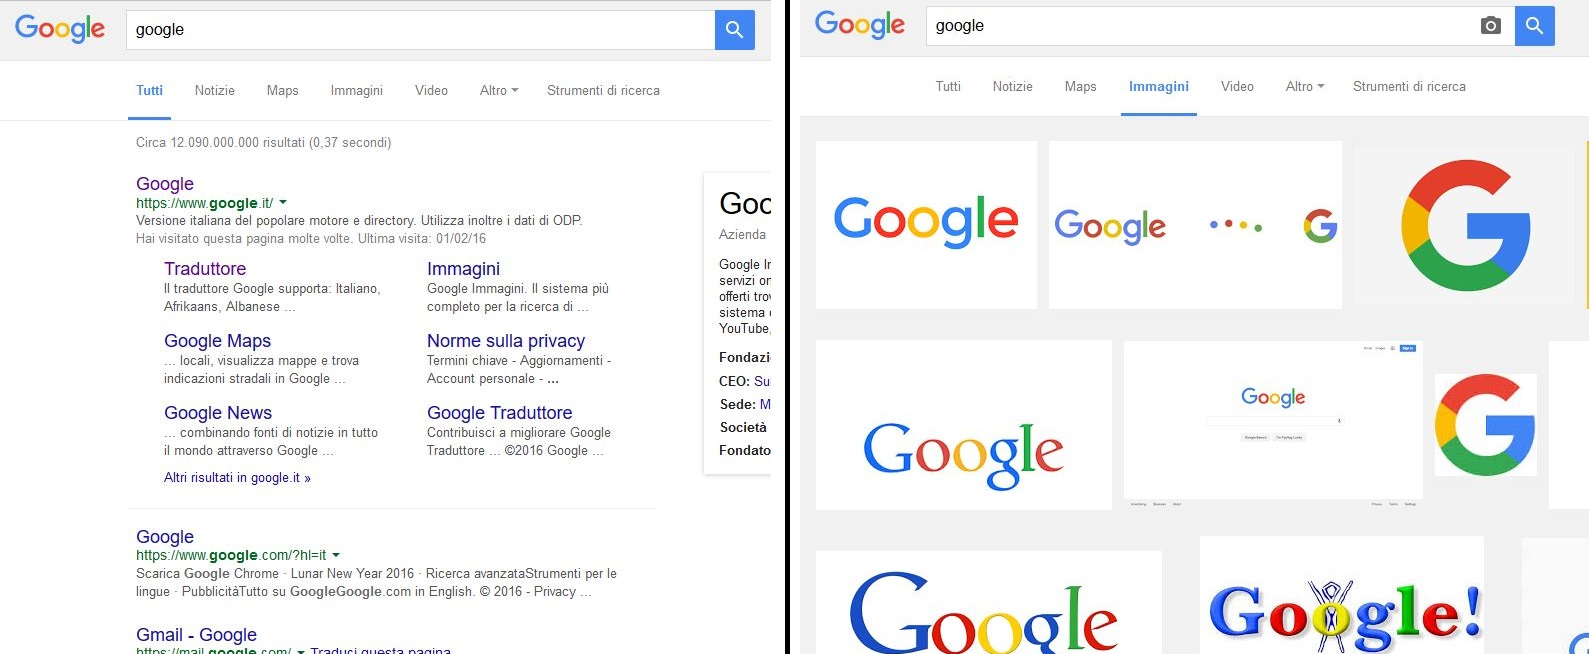
\includegraphics[width=\textwidth]{images/LaRicerca-Consigli}
			\caption[La ricerca - Tipi di presentazioni risultati]{La ricerca - Presentazione dei risultati lineare e a griglia}
			\label{fig:LaRicerca-Consigli}
		\end{figure}
		
	\section{Il search box}
		Agli arbori del web nelle caselle di ricerca si inserivano nella maggior parte dei casi parole uniche, con il passare del tempo però gli utenti usano sempre più parole. Il numero massimo di caratteri determina il numero di utenti a cui basterà.
		\begin{itemize}
			\item con 10 caratteri solo il 35\% degi utenti sarà soddisfatt.
			\item con 30 l'88\%.
		\end{itemize}
		Quest'ultimo numero è la media consigliata. Un box troppo piccolo aumenta lo stress proporzionalmente per ogni carattere che sfora e gli utenti tendono a scrivere meno con risultati della query più scarsi.
		Per la necessità di spazio per il design in molti casi si è ricorso ad un \textbf{box dinamico} che una volta cliccato si allarga per contenere più caratteri.
	
	\section{Ricerce 2.0 (*)}
		(N.B. la seguente sezione è incompleta)
		
		Il web è un media informativo visivo. Negli anni sono stati vari i tentativi di evolvere dal testo alla voce per un'interazione uomo-macchina di livello superiore. Esistono varie tecnologie:
		\begin{itemize}
			\item VoiceXML
			\item SSML
			\item PLS
			\item CCXML
			\item SRGS
		\end{itemize}
		che via via hanno migliorato l'interazione uomo macchina ma si è ancora lontani da \emph{HALL 9000} il supercomputer intelligente di \emph{2001: Odissea nello spazio}.
		
		\subsection{Il grande problema}
			Basarsi sulla voce non basta perché rende difficile interpretare le parole senza l'aiuto del \textbf{contesto}.
			La tecnologia \emph{Google Glass} non ha avuto successo proprio per questo motivo, l'utenza chiedeva più pulsanti perché la sintesi vocale non era ancora pronta.
			
		\subsection{L'utente e le ricerche 2.0}
			Le ricerche del 2.0 diminuiscono la soddisfazione del 42\%! Perché?
			\begin{itemize}
				\item Di fronte ad un assistente virtuale l'utente si forma aspettative più alte e per questo diventa ancora più esigente.
				\item Illudere l'utente presentando un robot simile all'umano non aiuta, molto meglio mantenere un'interfaccia robotica per non dare illusioni e creare grosse aspettative.
			\end{itemize}
			Un esempio positivo che segue questi accorgimenti è \emph{Anna} di IKEA. Vediamone i punti forti:
			\begin{itemize}
				\item riceve in input solo testo e presenta un engine linguistico ben fatto. 
				\item Ha un'interfaccia cartoon.
				\item È uno strumento facoltativo.
			\end{itemize}
		
		\subsection{Ivoluzione/evoluzione dell'interazione}
			Per il problema del contesto nei videogiochi si è sempre più limitata la libertà di scelta e interazione negli anni. Ciò perché un grado di libertà alto poteva generare incomprensioni tra utente e macchina e la frustrazione aumentava.
		
			\subsubsection{Il rumore}
				Un altro motivo per cui le interfacce non precise hanno un gradimento superiore è il rumore di fondo. È grazie al rumore di fondo che sembrano più naturali. A tal proposito si sono fatti studi sul rumore che costantemente viviamo. Esso ha una natura frattale ricorsiva e per generarlo basta continuare a \textbf{ridurre l'ampiezza} e \textbf{alzare la frequenza} e infine mettere insieme tutte le parti.
				Paradossalmente le interfacce imperfette danno più soddisfazione.